\chapter{Características de transferencia del JFET}
  En el análisis de los transistores de efecto de campo de juntura (JFET), resulta fundamental comprender la relación
  entre la tensión aplicada entre compuerta y fuente (\(V_{GS}\)) y la corriente de drenaje (\(I_D\)). Esta relación se
  conoce como característica de transferencia, ya que describe cómo la señal de entrada (voltaje de control)
  regula la corriente de salida del dispositivo.  

  La dependencia entre estas magnitudes está dada por la ecuación de Shockley, la cual permite predecir el
  comportamiento del JFET en la región de saturación. A partir de esta ecuación es posible determinar cómo varía \(I_D\)
  en función de \(V_{GS}\), estableciendo un modelo matemático que refleja el efecto de la compuerta sobre la conducción
  del canal:  

  \begin{equation}
    I_D = I_{DSS} \left( 1 - \frac{V_{GS}}{V_p} \right)^2
  \end{equation}
  
  A partir de los datos experimentales obtenidos en la curva de salida \(I_D(V_{DS})\), es posible determinar los
  valores de \(I_{DSS}\) y de la tensión de pinch-off \(V_p\). Con estos parámetros, se puede trazar la ecuación de
  Shockley y representar la característica de transferencia del JFET.  
  
  \begin{figure}[!ht]
    \centering
    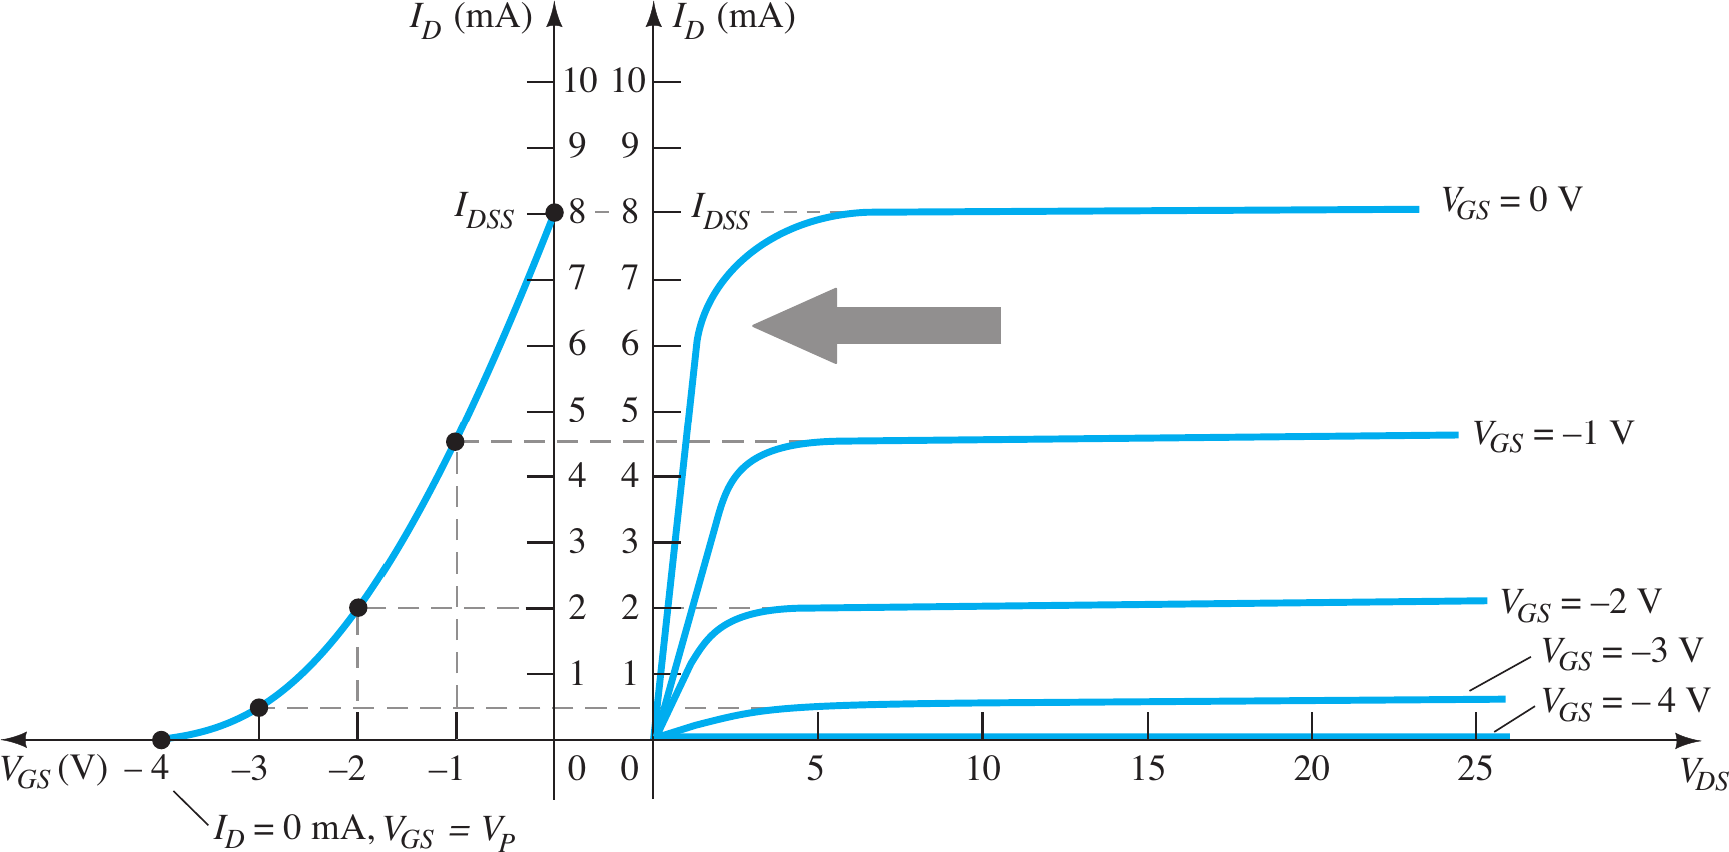
\includegraphics[width=1\textwidth]{images/grafico_transferencia.png}
    \caption{característica de transferencia del JFET obtenida a partir de la ecuación de Shockley.}
    \label{fig:transferencia}
  \end{figure}

\section{Actividad de Simulación}
    Se propuso implementar el circuito de la figura \ref{crkt:jfet-transf} en el simulador LTSpice, y hacer que la fuente
    $V2$ varíe desde $0V$ a $15V$ en pasos de $0.1V$, y por cada variación de la fuente $V2$, que la fuente $V1$ varíe de
    $0V$ a $8V$ en pasos de $0.1V$ para poder recrear una familia de curvas que expongan el comportamiento de la
    corriente $I_D$ en función del voltaje gate-source $V_{GS}$ por cada $V_{DS}$.
    \begin{figure}[!ht]
      \centering
      \begin{minipage}{0.45\textwidth}
        \begin{tikzpicture}
          % Paths, nodes and wires:
          \node[njfet](N1) at (2.25, 2.73){} node[anchor=west] at (N1.text){$2N5457$};
          \draw (4.75, 3.48) to[battery, l={$V2$}] (4.75, 1.98);
          \draw (4.75, 3.46) -- (4.75, 5.21) |- (2.25, 5.21) -| (2.25, 3.48);
          \draw (2.25, 1.96) -- (2.25, 0.73);
          \draw (4.75, 1.98) -- (4.75, 0.73);
          \node[ground] at (0.25, 0.73){};
          \node[ground] at (2.25, 0.73){};
          \node[ground] at (4.75, 0.73){};
          \draw (0.25, 1.25) to[battery, l={$V1$}] (0.25, 2);
          \draw (1.27, 2.46) -| (0.25, 2);
          \draw (0.25, 0.73) -| (0.25, 1.25);
        \end{tikzpicture}
        \caption{circuito de prueba para características de transferencia.}
        \label{crkt:jfet-transf}
      \end{minipage}
      \hfill
      \begin{minipage}{0.45\textwidth}
        \begin{lstlisting}[style=ltspice, caption={Parámetros de simulación LTspice}, label=list:jfet-transf]
.MODEL 2N5457 NJF IS=1N VT0=-1.5 BETA=1.125M LAMBDA=2.3M CGD=4PF CGS=5PF
.dc V1 0 3 .1 V2 0 15 .1
        \end{lstlisting}
      \end{minipage}
    \end{figure}

    \begin{figure}[!ht]
      \centering
      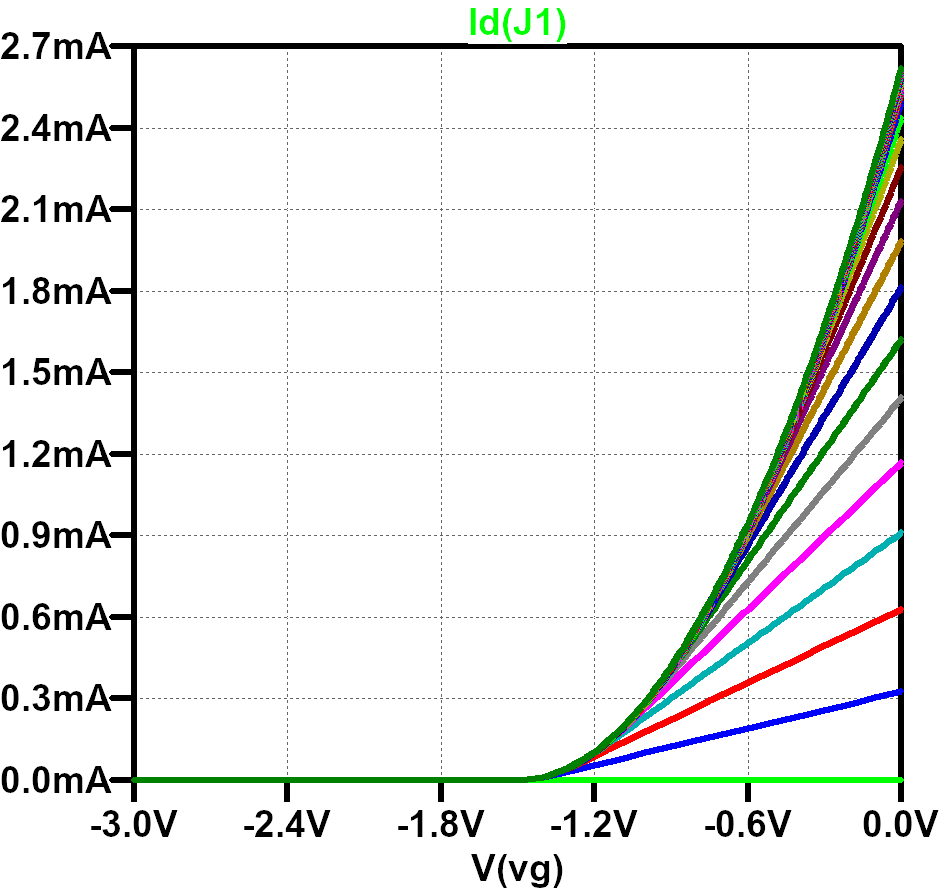
\includegraphics[width=0.65\textwidth]{images/transferencia-id_vds-vgs.png}
      \caption{resultados de simulación para características de transferencia del JFET.}
      \label{fig:sim.transf}
    \end{figure}

    Para poder apreciar mejor los resultados de la figura \ref{fig:sim.transf}, se redujo el barrido de la fuente $V1$
    hasta $3V$ en pasos de $0.1V$. Como se puede ver, el modelo describe perfectamente la familia de curvas de
    $I_{D_{(V_{GS}, \, V_{DS}})}$. La única diferencia observable comparada con la gráfica presentada por el fabricante es el
    valor de $I_{DSS}$.

\section{Actividad de Laboratorio}

    En esta actividad se implementó el circuito que se nos planteo con el objetivo de obtener las curvas características
    $I_{DS} = f(V_{GS})$ para distintos valores de $V_{DS}$.  El procedimiento consistió en fijar un valor de $V_{DS}$,
    variar la tensión $V_{GS}$ y medir los correspondientes valores de $I_{DS}$. Posteriormente, se cambió el valor de
    $V_{DS}$ y se repitió la medición, obteniendo así diferentes curvas que permiten observar el efecto del voltaje de
    compuerta en la corriente de drenaje.  
    
    Los valores experimentales obtenidos se resumen en la siguiente tabla:
    
    \begin{table}[h]
      \centering
      \resizebox{\textwidth}{!}{%
      \begin{tabular}{|c|c|c|c|c|}
        \hline
        \textbf{$V_{GS}$ [V]} & \textbf{$I_D$ [mA] ($V_{DS}=2$ V)} & \textbf{$I_D$ [mA] ($V_{DS}=5$ V)} & \textbf{$I_D$ [mA] ($V_{DS}=8$ V)} & \textbf{$I_D$ [mA] ($V_{DS}=15$ V)} \\ \hline
         0.0  & 0.98   & 1.31   & 1.59   & 2.11 \\ \hline
        -0.1  & 0.39   & 0.57   & 0.73   & 1.05 \\ \hline
        -0.2  & 0.07   & 0.137  & 0.146  & 0.16 \\ \hline
        -0.3  & 0.0043 & 0.0101 & 0.0183 & 0.0281 \\ \hline
        -0.4  & $\approx$0.003 & $\approx$0.003 & $\approx$0.003 & $\approx$0.003 \\ \hline
        -0.5  & 0.000  & 0.000  & 0.000  & 0.000 \\ \hline
        -1.0  & 0.000  & 0.000  & 0.000  & 0.000 \\ \hline
      \end{tabular}
      }
      \caption{corriente $I_D$ en función de $V_{GS}$ para $V_{DS}$ obtenidos experimentalmente.}
      \label{tab:ids-vgs-vds}
    \end{table}
    
    A partir de estos resultados es posible traficar el conjunto de curvas características del transistor y compararlas
    con las simulaciones y los valores obtenidos de la hoja de datos del fabricante.
    
    \begin{figure}[H]
      \centering
      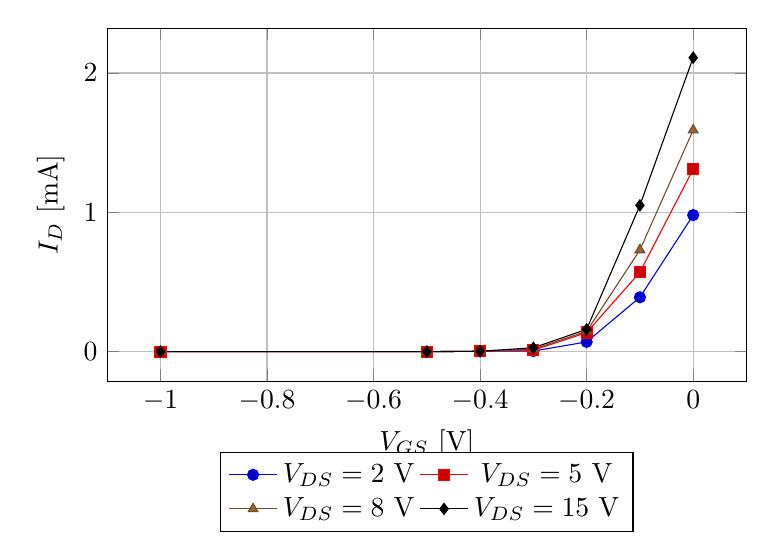
\begin{tikzpicture}
        \begin{axis}[
            grid=major,
            xlabel={$V_{GS}$ [V]},
            ylabel={$I_{D}$ [mA]},
            legend style={at={(0.5,-0.2)},anchor=north,legend columns=2},
            width=0.8\textwidth,
            height=0.5\textwidth,
        ]
        
        \addplot+[mark=*] coordinates {
        (0.0,0.98) (-0.1,0.39) (-0.2,0.07) (-0.3,0.0043) (-0.4,0.003) (-0.5,0) (-1.0,0)
        };
        \addlegendentry{$V_{DS}=2$ V}
        
        \addplot+[mark=square*] coordinates {
        (0.0,1.31) (-0.1,0.57) (-0.2,0.137) (-0.3,0.0101) (-0.4,0.003) (-0.5,0) (-1.0,0)
        };
        \addlegendentry{$V_{DS}=5$ V}
        
        \addplot+[mark=triangle*] coordinates {
        (0.0,1.59) (-0.1,0.73) (-0.2,0.146) (-0.3,0.0183) (-0.4,0.003) (-0.5,0) (-1.0,0)
        };
        \addlegendentry{$V_{DS}=8$ V}
        
        \addplot+[mark=diamond*] coordinates {
        (0.0,2.11) (-0.1,1.05) (-0.2,0.16) (-0.3,0.0281) (-0.4,0.003) (-0.5,0) (-1.0,0)
        };
        \addlegendentry{$V_{DS}=15$ V}
        
        \end{axis}
      \end{tikzpicture}
      \caption{$I_{D}$ en función de $V_{GS}$ para distintos valores de $V_{DS}$.}
    \end{figure}

